\documentclass{article}

\usepackage[utf8]{inputenc}
\usepackage{CJKutf8}
\newenvironment{Korean}{%
 \CJKfamily{mj}}{}

\usepackage{natbib}
\usepackage{graphicx}
\usepackage{amssymb}
\setcounter{tocdepth}{3}
\usepackage{graphicx}
\usepackage{subfigure}
\usepackage{mathtools}
\usepackage{cite}
\usepackage{multirow,makecell}
\usepackage{listings}
\usepackage{titlesec}
\usepackage{booktabs}
\setcounter{secnumdepth}{4}

\begin{CJK}{UTF8}{}
\begin{Korean}

\title{RE510 Intelligent Robot Design Lab. HW 1}

\author{Hyungtae Lim}

\date{20th, March, 2019}

\titleformat{\paragraph}
{\normalfont\normalsize\bfseries}{\theparagraph}{1em}{}
\titlespacing*{\paragraph}
{0pt}{3.25ex plus 1ex minus .2ex}{1.5ex plus .2ex}

\begin{document}
\maketitle


\section{Introduction}

본 실험에서는 Unified Robot Description Format (URDF)를 통해  two-wheeled 모바일 로봇을 구현하여 Gazebo로 시뮬레이션을 실행시키고 Gazebo로 topic publish하여 제어하는 것을 목적으로 한다. URDF에서 two-wheeled 로봇에 필요한 Chassis,  LeftWheel, RightWheel를 생성하는데 필요한 parameter를 URDF로 설정한 후 Joint를 통해 바퀴와 몸체를 연결 시켰다. 제작한 모바일 로봇을 ROS launch로 구동할 수 있게 hw1.launch file을 작성하였고, rostopic 명령어를 통해 geometry\underline{ }msgs를 publish하여 two-wheeled 로봇을 조종해보았다.

\section{Experiment Implementation}

\subsection{ROS Package}

먼저 ROS package를 위한 RE510\underline{ }ws라는 workspace를 생성한 후, 그 후 build를 해주었다. package를 위한 폴더가 다 생성되었다는 가정 하에 아래와 같이 실행하였다. catkin\underline{ }create\underline{ }pkg 명령어를 통해 std\underline{ }msgs, rospy, roscpp을 import해온 hw1 package를 생성하였다. 실험에 사용된 컴퓨터에서는  catkin-tools를 설치하여 사용하고 있기 때문에 기존의 catkin\underline{ }make가 아닌 catkin build 명령어를 통해 ROS package를 build한다. 마지막으로 linux에서 기본으로 제공하는 bash shell을 쓰지 않고 oh-my-zsh를 쓰기 때문에 shell 파일을 zsh에 맞춰서 setup.zsh 파일을 source해줘야 한다. 코드 명령어는 다음과 같다. 

\begin{lstlisting}[frame=single]
$ cd ~/RE510_ws/src
$ catkin_create_pkg hw1 std_msgs rospy roscpp
$ cd ..
$ catkin build
$ source devel/setup.zsh

\end{lstlisting}

\subsection{Unified Robot Description Format}

URDF에서는 원하는 물체는 link를 통해 생성하고 joint를 통해 각각 link들을 연결한다. 본 실험에서는 로봇의 몸체(Chassis), 왼쪽 오른쪽 바퀴(LeftWheel, RightWheel)를 link로 생성하였고 joint로 각각 로봇의 왼쪽과 오른쪽에 바퀴를 각각 연결해주었다.   

\subsubsection{Link}

Link는 크게 물체의 inertial property를 기술하는 $\langle$intertial$\rangle$, simulation 상에서 visualization을 위해 사용되는 $\langle$visual$\rangle$, 물리 엔진 상에서 고려되는 $\langle$collision$\rangle$으로 구성된다. 형체가 복잡한 모델인 경우에는 simulation 상에서 물리 엔진의 computational complexity를 낮추기 위해 $\langle$collision$\rangle$을 구성할 때 $\langle$visual$\rangle$에서 좀 더 단순화하여 모델링한다. 하지만 본 실험의 경우에는 two-wheeled 로봇이 단순히 두개의 cylinder와 하나의 box로 구성되어 있기 때문에 Chassis, LeftWheel, RightWheel 모두 $\langle$visual$\rangle$과 $\langle$collision$\rangle$을 같게 설정해주었다.

\paragraph{Chassis}

Chassis의 무게를 $m_{body}$라고 하고, 가로, 세로, 높이의 길이를 각각 $a$, $b$, $c$ 가로 높이로 구성된 평면을 수직으로 지나는 선을 x, 세로와 높이로 구성된 평면을 수직으로 지나는 선을 y, 가로와 세로 면을 수직으로 지나는 선을 z축으로 하게 되면 각각의 moment of inertia는 다음과 같다. 

\begin{align}
I_{xx} & =\frac{m*(a^2 + c^2)}{12} \\ 
I_{yy} & =\frac{m*(b^2 + c^2)}{12} \\
I_{zz} & =\frac{m*(a^2 + b^2)}{12} 
\end{align}
\begin{align}
I_{xx} & = I_{yy} = \frac{m*(3r^2 + h^2)}{12} \\ 
I_{zz} & =\frac{m*r^2}{2} 
\end{align}
그리고 Chassis가 이 모델에서 중심이기 때문에 chassis의 위치를 $\left\{x, y, z, r, p, y\right\}=\left\{0, 0, 0, 0, 0, 0\right\}$로 잡았다. 본 실험에서는 $a=b=0.3m$, $c=0.05m$로 설정하여 chassis를 구성하였다. 그리고 처음에는 $m_{body}=5kg$로 하였다. 따라서 $I_{xx}=I_{yy}=0.0386kg*m^{2}$,  $I_{zz}=0.075kg*m^{2}$임을 알 수 있다.

\paragraph{Wheels}

왼쪽과 오른쪽의 바퀴는 모두 형태가 동일하기 때문에 한꺼번에 wheel이라 총칭하고 설명한다. Wheel의 무게를 $m_{wheel}$라고 하고, 반지름과 높이의 길이를 각각 $r$, $h$라 할 때 원기둥의 원면을 수직으로 지나는 선을 z, 원z과 수평하게 지나고 원기둥의 옆면을 수직으로 지나가는 선을 각각 x, y축으로 잡으면 각각의 moment of inertia는 다음과 같다.

\begin{align}
I_{xx} & = I_{yy} = \frac{m*(3r^2 + h^2)}{12} \\ 
I_{zz} & =\frac{m*r^2}{2} 
\end{align}

본 simulation에서는 $r=0.1m$, $h=0.05m$로 설정하여 wheel를 구성하였다. 그리고 $m_{wheel}=3.5$로 지정하였다. 따라서 $I_{xx}=I_{yy}=0.00948kg*m^{2}$, $I_{zz}=0.0175kg*m^{2}$임을 알 수 있다. Wheels는 chassis의 옆부분에 달아야하므로 $\left\{x, y, z, r, p, y\right\}=\left\{0, 0, 0, 1.5708, 0, 0\right\}$로 roll 방향으로 90도 회전시켜 주었다.

\subsubsection{Joint}

Joint는 위에서 만든 Chassis와 Wheel을 연결시켜주는 역할을 한다. Chassis에 오른쪽 바퀴를 연결시킬 joint와 왼쪽 바퀴를 연결시킬 joint가 각각 필요하다. Joint를 연결하기 위해서는 각각 parent link와 child link를 지정하고 joint의 각도와 위치를 지정해주어야 한다. 본 실험의 경우 LeftWheelJoint와 RightWheelJoint 총 2개의 joint가 사용되었다. 둘 다 parent link는 Chassis이지만, LeftwheelJoint의 child는 LeftWheel, RightwheelJoint의 child는 RightWheel로 설정해주었다. Joint의 origin은 Chassis의 옆쪽인 $\pm$0.175m에 부착하였다. $($LeftWheelJoint가 -$)$ 마지막으로 wheel과 축을 맞추기 위해 joint의 축을 $\left\{x, y, z, r, p, y\right\}=\left\{0, 1, 0, 0, 0, 0\right\}$으로 맞추었다.

% Joint의 type은 처음에 회전을 하기 때문에 revolute로 설정하였는데, 시행작오를 통해 continous로 설정해야 한다는 것을 확인했다. 

\subsubsection{Differential Drive Controller}

Gazebo를 실행시키는데 필요한 변수와 control에 필요한 변수들은 선언해 주었다. 굉장히 많은 변수의 값들을 지정해주었는데, 주요 변수는 다음과 같다. Two-wheeled 로봇을 rostopic으로 직접 구동하면서 잘 움직이는 변수를 경험적으로 찾아 적용하였다. wheelTorque와 wheelAcceleration이 작으면 주어진 rostopic pub pub 명령어에 필요한 속도에 빠르게 도달하지 못 할 것 같아 적절히 큰 값으로 지정하였다. 

\begin{table}[h]
	\centering
	\caption{Important options that are needed to operate Gazebo among all options}
	\begin{tabular}{cc}
		\toprule
		Option name     &  Value   \\ \midrule
		updateRate     & 100 \\
		LeftJoint     & LeftWheelJoint \\
		RightJoint     & RightWheelJoint \\
		wheelSeparation     & 0.35 \\
		wheelDiameter    & 0.2 \\
		wheelTorque     & 300 \\
		wheelAcceleration     & 20 \\
		commandTopic     & cmd\underline{ }vel \\ \bottomrule
	\end{tabular}
	\label{table:rmse}
\end{table}

\subsection{Commands for Launching a ROS Launch File and Publishing a Topic}

ROS launch file에는 Gazebo의 빈 world map을 include하는 내용과 URDF로 생성한 model을 불러오는 내용을 작성해야 한다.
따라서 hw1.launch에 아래와 같은 내용을 추가 작성해주었다.

\begin{lstlisting}
<include file="$(find gazebo_ros)/launch/empty_world.launch">
<node name="urdf_spawner" pkg="gazebo_ros" type="spawn_model"
 respawn="false" output="screen" args="-urdf -model mybot -file
 $(find hw1)/urdf/two_wheeled_robot.urdf"/>
\end{lstlisting}

ROS launch file을 실행시키는 command와 /cmd\underline{ }vel을 publish하는 command는 아래와 같다. 아래의 -r option은 hz를 설정해주는 option이다. default hz가 10이기 때문에 굳이 command line에 추가를 해주지 않아도 된다. 
 
\begin{lstlisting}[frame=single]
$ roslaunch hw1 hw1.launch
---------------Open another terminal---------------
$ rostopic pub /cmd_vel geometry_msgs/Twist "linear:
 x: 2.0
 y: 0.0
 z: 0.0
angular:
 x: 0.0
 y: 0.0
 z: 1.8" -r 10
\end{lstlisting}

\section{Experimental Results}

작성된 URDF 파일과 launch file로 실행된 Gazebo에서 지정한 물체들이 잘 형성되었는지와 publish된 topic로 잘 움직이는 지 확인해보았다.

\subsection{Pakage Composition}

Chapter 2.1과 2.3을 통해 생성된 파일들을 확인해 보면 RE510\underline{ }ws$/$src에 hw1라는 폴더가 생성되었고 이 폴더에는 각각 launch file이 담긴 launch 폴더와 two-wheeled 로봇의 URDF가 담긴 urdf 폴더, build할 때 종속되어지는 package들이 들어있는 CMakeLists.txt, package의 메타정보를 지니는 package.xml가 생성됨을 아래와 같이 확인할 수 있다.

\begin{lstlisting}
~/RE510_ws/src/hw1/
    -launch
        - -hw1.launch
    -urdf
        - -two_wheeled_robot.urdf
    -CMakeLists.txt
    -package.xml
\end{lstlisting}

\subsection{Robot Properties}

 Figure. \ref{fig:architecture}에서 볼 수 있듯이 mybot이라는 model에 Chassis, LeftWheel, RightWheel, LeftWheelJoint, RightWheelJoint가 잘 생성된것을 확인할 수 있었다.

\begin{figure}[h]
	\centering
	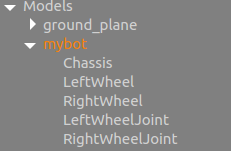
\includegraphics[width=3.5cm]{materials/architecture1}
	\caption{Hierarchy of the URDF model.}
	\label{fig:architecture} 	
\end{figure}

\subsubsection{Chassis}

Figure. \ref{fig:experimental_envorinment}에서 확인할 수 있듯이, BOX의 크기가 0.3*0.3*0.05로 잘 형성된 것을 확인했다. 또한 $m=20$에 따른 moment of inertia 또한 맞는 값으로 입력되었음을 확인했다.

\begin{figure*}[h]
	\centering
	\subfigure[]{\label{fig:chassis_geometry} 		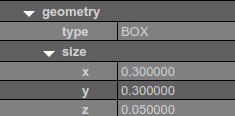
\includegraphics[height=2.5cm]{materials/chassis_geometry}
	}
	\subfigure[]{\label{fig:chassis_inertial} 		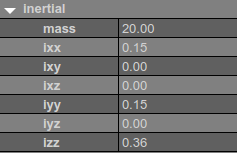
\includegraphics[height=2.5cm]{materials/chassis_inertial}
	}
	\caption{(a) Geometry of Chassis. (b) Moment of inertia of Chassis. }\label{fig:experimental_envorinment}
\end{figure*}


\subsubsection{Wheels}

Figure. \ref{fig:wheel}에서 확인할 수 있듯이, BOX의 크기가 $r=0.1$, $h=0.05$로 잘 형성된 것을 확인했다. 또한 $m=3.5$에 따른 moment of inertia 또한 맞는 값으로 입력되었음을 확인했다.

\begin{figure*}[h]
	\centering
	\subfigure[]{\label{fig:wheel_geometry} 		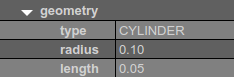
\includegraphics[height=2.5cm]{materials/wheel_geometry}
	}
	\subfigure[]{\label{fig:wheel_inertial} 		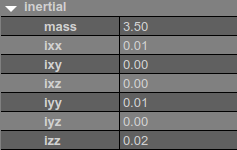
\includegraphics[height=2.5cm]{materials/wheel_inertial}
	}
	\caption{(a) Geometry of wheels. (b) Moment of inertia of wheels. }\label{fig:wheel}
\end{figure*}


\subsubsection{Joint}

Joint의 property를 통해 parent link와 child link가 잘 연결되어 있는지 확인할 수 있다. Figure. \ref{fig:joint}에서 볼 수 있듯이 parent link가 Chassis로, child link가 LeftWheel에 잘 연결되어 있는 것을 확인할 수 있다. RightWheel도 마찬가지로 parent link가 Chassis로, child link가 RightWheel로 연결된다.

\begin{figure}[h]
	\centering
	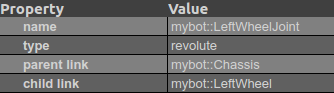
\includegraphics[height=2.5cm]{materials/joint_constraint}
	\caption{Property of LeftWheelJoint.}
	\label{fig:joint} 	
\end{figure}

\subsection{ROS Topic}

Section 2.3에서 rostopic으로 publish된 topic이 어떻게 전달되고 있는지는 다음과 같은 명령어로 확인할 수 있다.

\begin{lstlisting}[frame=single]
$ rqt_graph
\end{lstlisting}

\ref{fig:rqt_graph}에서 볼 수 있듯이, Section 2.3에서 중복을 피하기 위해 익명으로 publish된 rostopic /cmd\underline{ }vel이 publish되어 /gazebo를 가르키는 것을 확인할 수 있다.

\begin{figure}[h]
	\centering
	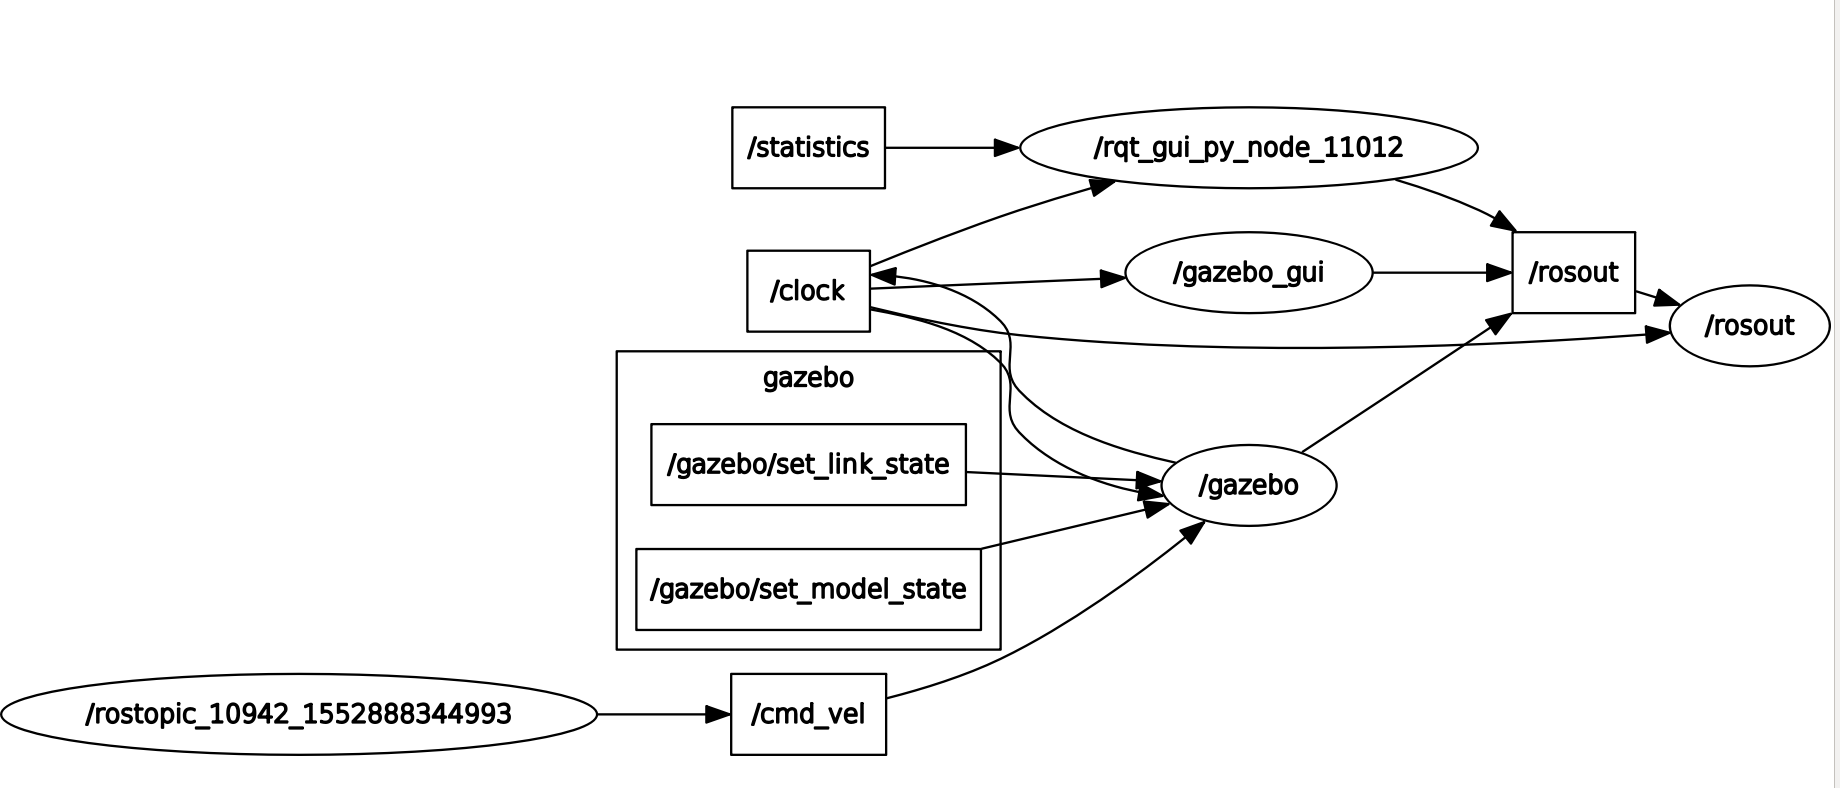
\includegraphics[width=0.9\linewidth]{materials/rqt_graph}
	\caption{A graph that the relationships between each ROS topics are described.}
	\label{fig:rqt_graph} 	
\end{figure}

Figure. \ref{fig:rqt_graph}는 ROS 상에서 각각 publish하는 node들과 subscribe하는 node들을 그래프화하여 명시해준다. 보는 바와 같이 ROS launch로 실행된 set\underline{ }link\underline{ }state와 set\underline{ }model\underline{ }state가 /gazebo로 publish되는 것을 확인할 수 있다. 또한 rostopic으로 publish되는 topic들도 /gazebo로 전달되는 것을 확인할 수 있다.

\section{Conclusion}

본 실험에서는 URDF를 이용하여 직접 two-wheeled 로봇을 만들어보았고 ROS launch 를 통해 Gazebo simulation을 실행시키고 rostopic command를 통해 제작한 로봇을 구동해 보았다. ROS package를 생성한 후 URDF에서 모바일 로봇의 Chassis, Wheels를  $\langle$visual$\rangle$, $\langle$inertial$\rangle$, $\langle$collision$\rangle$에 따라 필요한 property를 지정해주었고 LeftWheelJoint와 RightWheelJoint를 통해 Chassis와 Wheel들을 연결시켜 주었다. 그 후 각 값들이 실제 적용됨을 Gazebo를 통해 확인할 수 있었다. 

ROS launch로 Simulation을 실행시킨 후 rostopic command를 통해서 10hz로 로봇이 원운동을 하게 명령을 주었다. publish되는 topic에 따라 생성된 로봇이 잘 작동됨을 확인할 수 있었다. 하지만 가끔 Chassis가 바닥에 부딪칠 때 몸체가 뒤집혀버리는 문제가 발생하는 것을 확인했다. Two-wheeled 로봇의 특성 상 두 바퀴로만 균형을 잡기 때문에 운동 중에 Body가 기울거나 바닥에 부딪히는 상황이 발생하는 것이다. 

이를 해결해주기 위해서는 몸체의 기우는 정도도 parameter로 받아와서 feedback control을 통해 PID control을 하는 node도 따로 하나 더 생성하여 움직임과 동시에 chassis의 기울기도 동시에 제어를 하면 해결할 수 있다. 혹은 하드웨어적으로 뒷부분에 caster를 부착하면 좀 더 안정적인 상태로 움직일 수 있을 것으로 보인다.

\section{Reference}

.

[1] ROS.org., urdf/XML/joint. http://wiki.ros.org/urdf/XML/joint

[2] ROS.org., urdf/XML/line. http://wiki.ros.org/urdf/XML/line

[3] GAZEBO, Tutorial: Using a URDF in Gazebo. \\ http://gazebosim.org/tutorials?tut=ros\_urdf\&cat=connect\_urdfros

[4] ROS.org., ros\_control. http://wiki.ros.org/ros\_control
\end{Korean}
\end{CJK}

\end{document}
